\documentclass[hidelinks, 12pt, oneside]{article}
\usepackage{bookmark}
\usepackage{graphicx}
\usepackage{hyperref}
\graphicspath{{images/}}
\usepackage[utf8]{inputenc}
\usepackage[english]{babel}
\begin{document}

 %titlepage
\thispagestyle{empty}
\begin{center}
\begin{minipage}{0.75\linewidth}
    \centering
    
 {\normalsize Project Tender\par}
 \vspace{1cm}
%Thesis title
    {\uppercase{\Large Project Name: Cafeteria Management System.\par}}
   	{\Large Client: Resolve\par} 
    \vspace{1cm}

%Thesis title
    {\uppercase{\Huge Group Name\par}} 

%Author's name
    {\Large Rendani Dau 13381467\par}
    {\Large Elana Kuun u12029522\par}
    {\Large Semaka Malapane 13081129 \par}
    {\Large Antonia Michael 13014171\par}
    {\Large Isabel Nel 13070305\par}
    \vspace{1cm}
    
\end{minipage}
\end{center}
\clearpage

\tableofcontents

\newpage
\section{The Team}

\subsection{Antonia Michael}
 
\begin{figure}[h!]
  \centering
    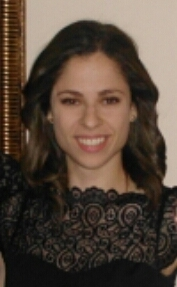
\includegraphics[width=0.85\textwidth]{t} 
\end{figure}

\subsubsection{Interests}
My interests include working with people, helping people, reading, tennis, greek dancing. 
\subsubsection{Technical Skills}
My technical skills include: Java, C++, Html5, css, php, Bootstrap, Javascript, Semantic UI, Sql, php, python,  WebGL, Latex, Github, shell script, AngularJS, NodeJS, Microsoft Office, Npm, HandleBars Server, Mongoose, Gemfury. 
\subsubsection{Past experiences relevant for project}
Programming \\
I have done an internship at a small IT company called Lepsta (Pty)Ltd, where I worked mainly on the front end of their new systems. I was mainly responsible to implement the gui and front end functionality of their email client app called Ridicle, using AngularJS, Python, Semantic UI, and using Brackets as the platform.
I also assisted in implementing a CMS Website for small enterprise, NCC Solutions. In addition, for COS 301 I was chosen to be part of the Infrastructure Integration team to integrate the code given to us from the functional teams. We used NodeJS, RoboMongo, Mongoose, Nodemailer, Npm, Gemfury and HandleBars server for our integration. \\

Business Analysis \\
I also worked as a business analyst at Lepsta (Pty)Ltd, where my duties included firstly, requirements management - gathering, defining, analyzing and documenting business and functional requirements and designing a solution based on these requirements. Secondly, communicating requirements to programmers and other stakeholders ensuring that everyone understands what is required for the project to be a success. I also had to develop the business processes to provide a graphical flow of data, indicating the relationship between stakeholders and systems. I had to also design the test cases and implement the testing. Throughout the process I served as a communication channel, ensuring that all the teams knew exactly what was expected of them, and reported their progress and any concerns to me.
\\
Project Management \\
At Lepsta (Pty)Ltd I also worked as a Project Manager. I developed a schedule for the project completion, allocating resources to the tasks. I also had to determine resources needed to complete the different phases of the project (i.e. time, money, technologies). I used a Gannt chart to allocate time frames for the different tasks in the project. I used a SCRUM board to keep track of the progress of the different tasks and to let the project needs see a visual representation of their tasks at hand. I had to keep regular communication with management to express the programmers' concerns and progress. It was also my job to develop team spirit and make sure that each member is contributing equally to the projects. \\
 
\subsubsection{Non technical strengths}
My non technical strengths include: \\

Leadership skills - 
 \\1.) Head of Communications in The School of IT faculty House
 \\2.) Selected by the Department of Computer Science to be a 	Infrastructure Team Leader for the module COS 301 for the implementation of The Buzz System, 
 \\3.) Was a class Representative for the module, Imperative Programming.
   
Public speaking and presentation skills - Got chosen as the best overall paper and presentation from our presentation at the 2014 ACEIE Information Science Conference held at The University of Pretoria. Was then selected by UP to present research paper at the 2014 Information Ethics Conference held at The University of Zululand, competing with students from UJ, UP and other universities. We obrained 2nd place. 
\\
Social responsibility skills - Tutored for the Basic Computer Training course (6 sessions) for underprivileged female students eager to persue IT careers.\\ 
Organised and ran a Computer Training course for members of the community at UP Mamelodi Campus with a group of 4 other students - 40 hours of community work for JCP community development module in second year \\

Debutantes Year at school (2010) – Hosted various events/ programmes to raise funds for the Phehela Day and Night Centre and assisted with other similar charities.\\,

Teaching skills - In addition, the computer literacy courses I have taught, I am currently a Tutor in the Computer Science Department at the University of Pretoria.
Other skills: 
Communication skills, team work skills and people skills.

\subsubsection{What makes you want to do the project} 
Will complete this soon
\\

\subsection{Rendani Dau}
\subsubsection{Interests}
\subsubsection{Technical Skills}
\subsubsection{Past experiences relevant for project}
\subsubsection{None technical strengths}
\subsubsection{What makes you want to do the project}

\subsection{Elana Kuun}
\subsubsection{Interests}
\subsubsection{Technical Skills}
\subsubsection{Past experiences relevant for project}
\subsubsection{None technical strengths}
\subsubsection{What makes you want to do the project}

\subsection{Semaka Malapane}

\begin{figure}[h!]
  \centering
    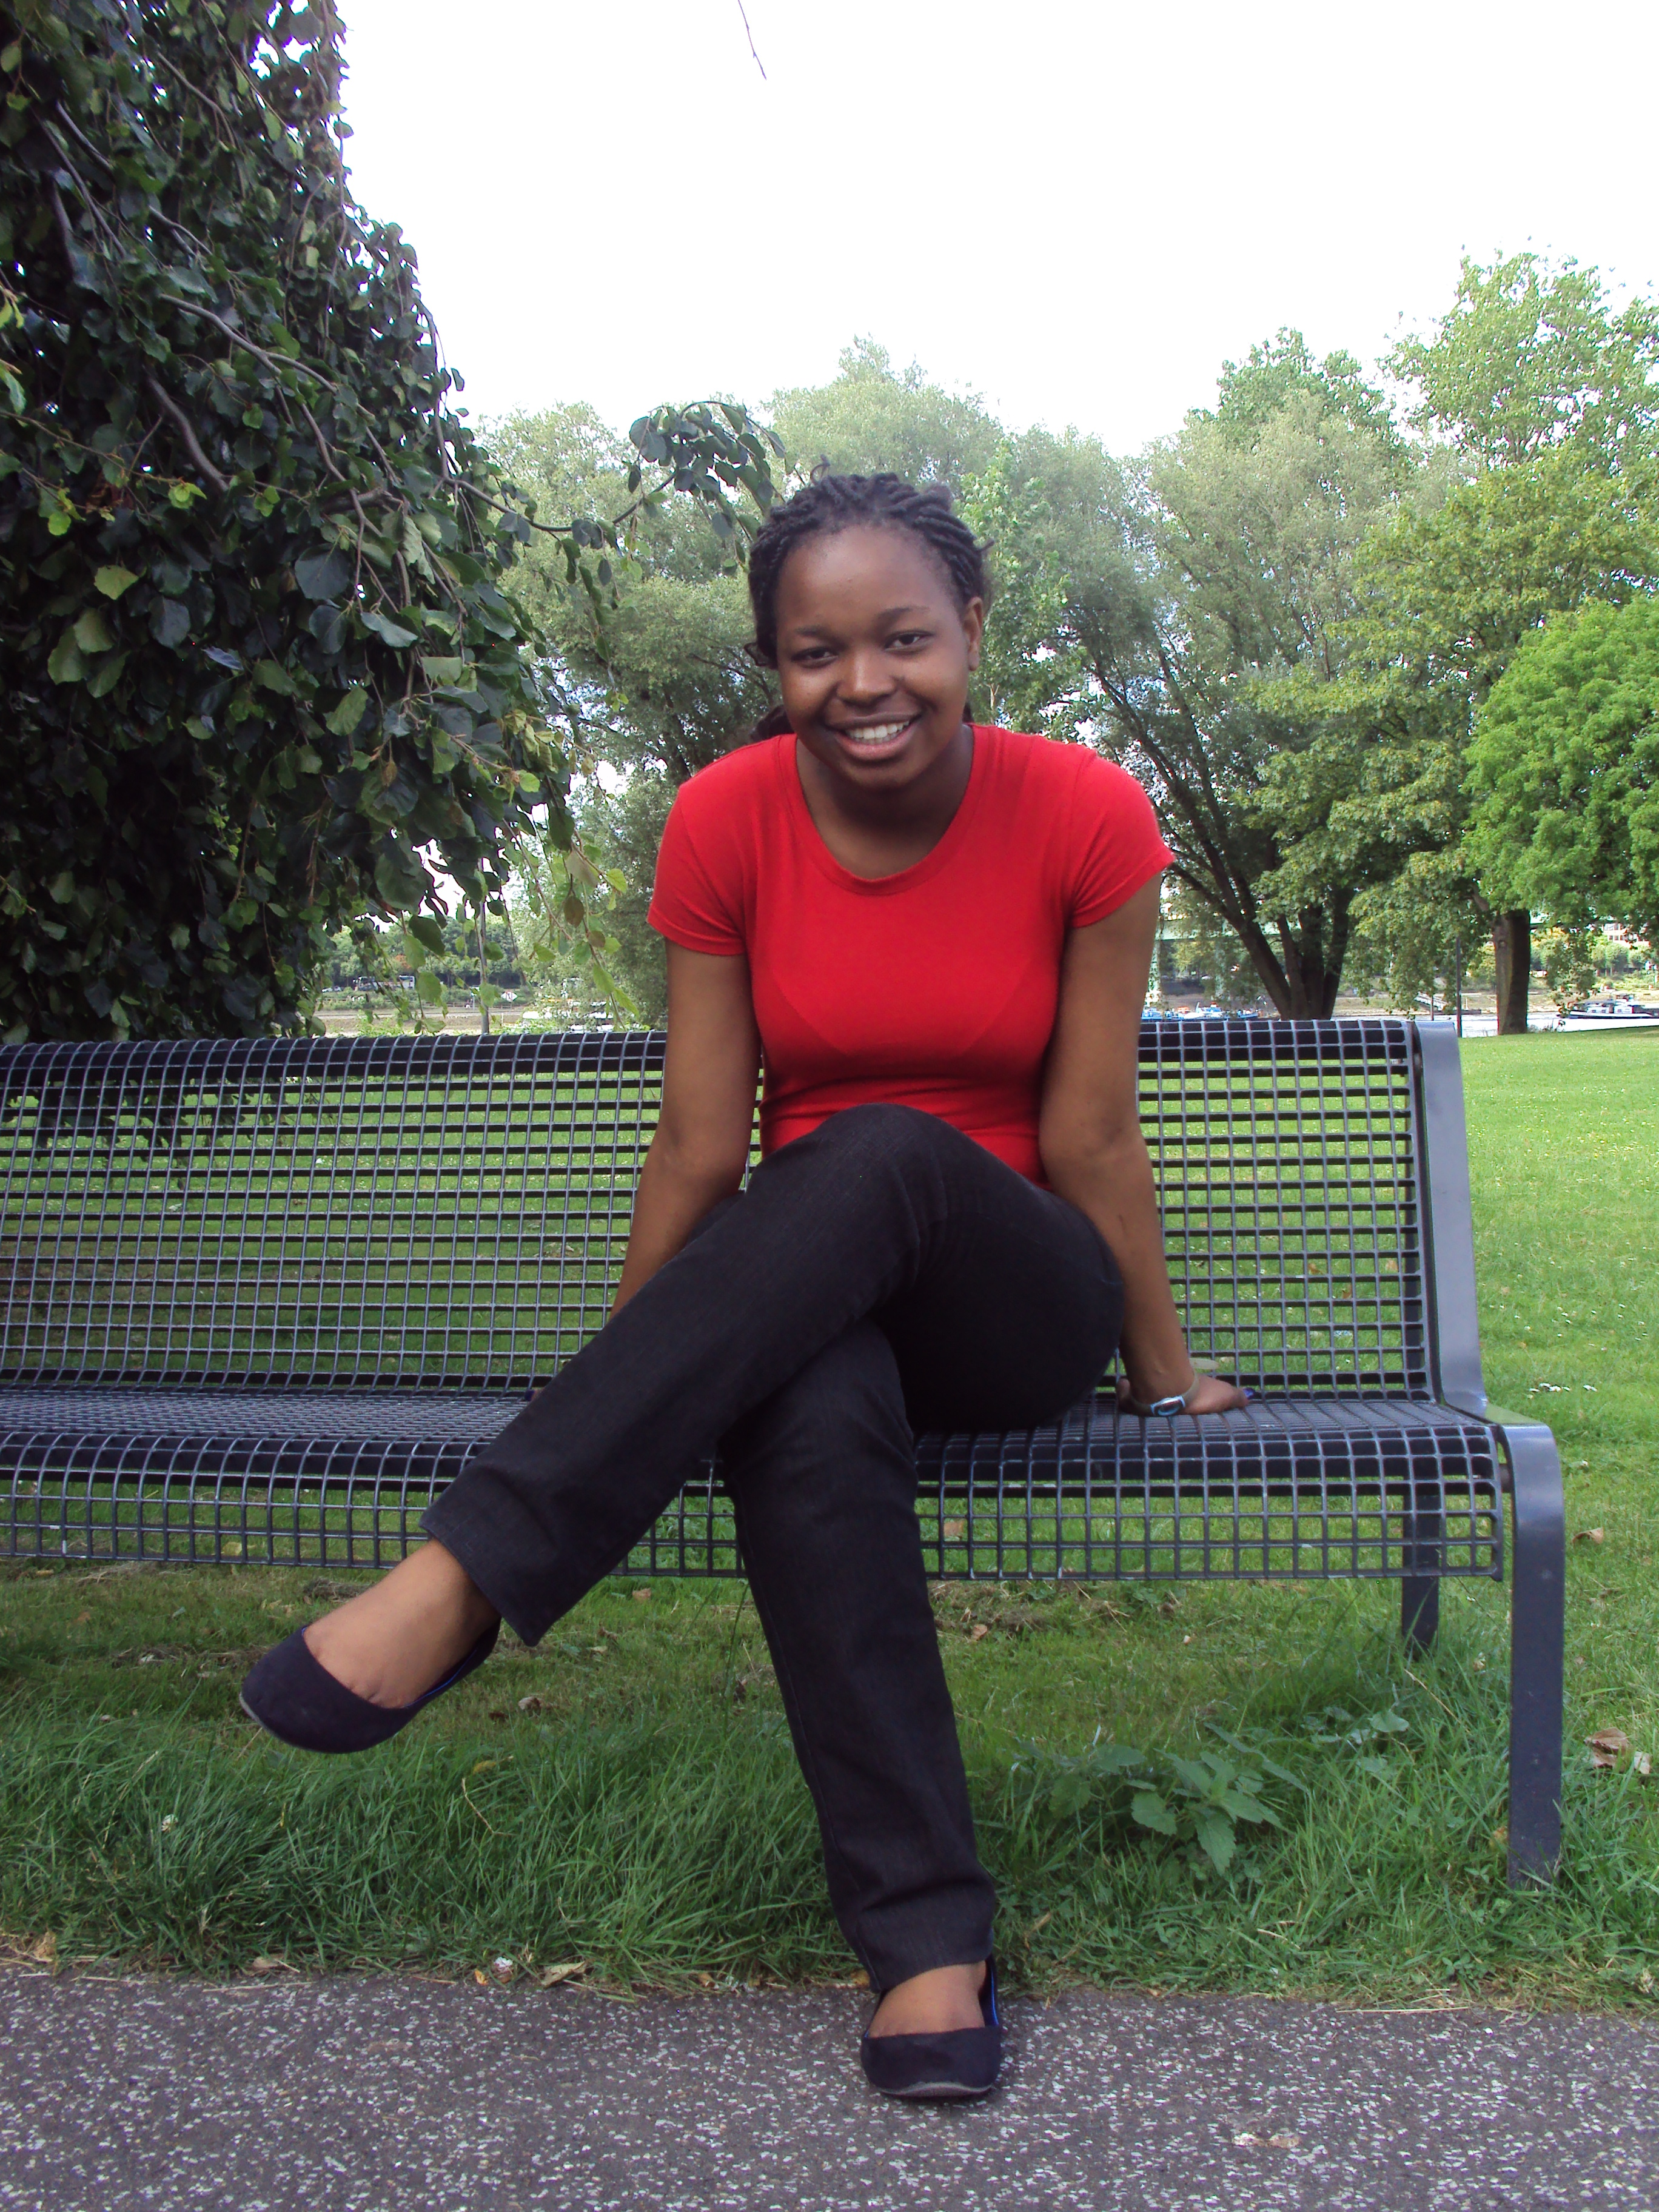
\includegraphics[width=0.85\textwidth]{Semaka} 
\end{figure}

\subsubsection{Interests}

My interests are playing sudoku, cards, cooking, reading, shopping and spending time with friends and family.

\subsubsection{Technical Skills}

My technical skills include: C++, Java, CSS, PHP, HTML, JavaScript, NodeJS, Mongoose, WebGL, Microsoft Office, SQL and XML.
 
\subsubsection{Past experiences relevant for project}

I have successfully completed database management and design. Not only did I enjoy the module but it taught me the required skills - SQL and databases - for this project. 

\subsubsection{Non technical strengths}

My non technical strengths include: 

Team work and communication skills - The Software Engineering course offered us a mini project at the beginning of the year where we had to work in multiple different teams with different kinds of people. This gave me the opportunity to learn to work in a team setting and to communicate appropriately.
 
Public speaking and presentation skills - I participated in public speaking in 2011 and 2012. This taught me not only good speech writing but valuable presentation skills.
I also took part in a computer training course at the UP Mamelodi Campus in 2014 - this gave me the opportunity to better my public speaking and presentation skills.

Social responsibility skills - I tutored a Basic Computer Training course (6 sessions) for underprivileged female students.
I organised and ran a Computer Training course for members of the community at UP Mamelodi Campus with a group of 4 other students - 40 hours of community work for JCP community development module in second year.

\subsubsection{What makes you want to do the project}

This project seems like an interesting challenge. It will give us exposure to working with databases, which we aren't often exposed to. It will also be exciting at the end of the year to be able to see the end product of this working program.

\subsection{Isabel Nel}

\begin{figure}[ht!]
\centering
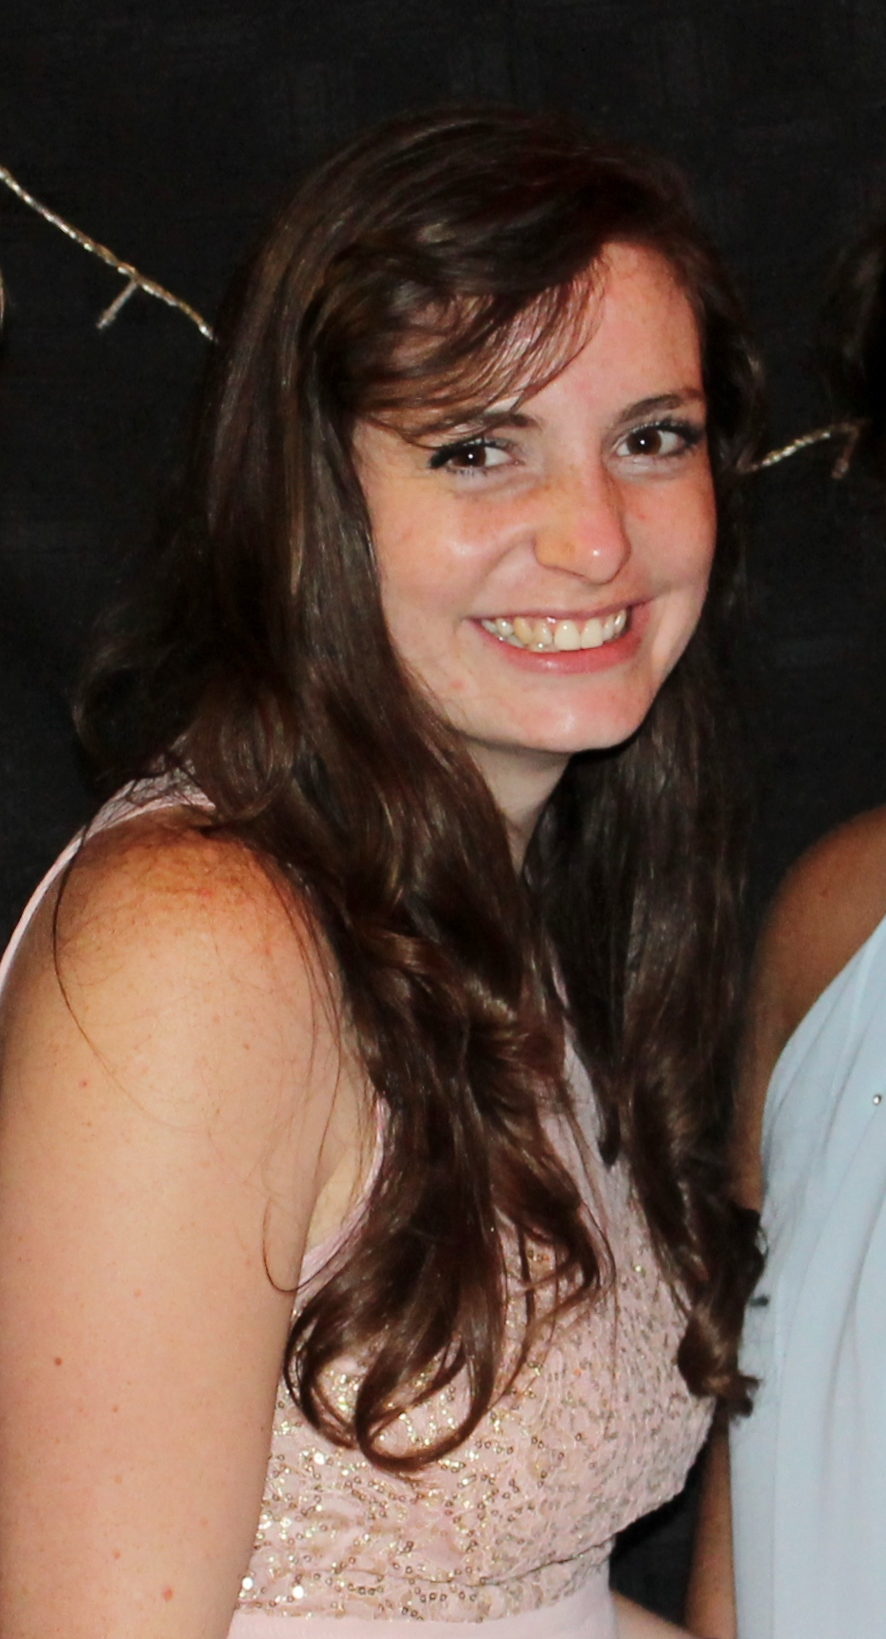
\includegraphics[width=50mm]{IsabelNel.jpg}
\end{figure}

\subsubsection{Interests}
During my past two years of studying Computer Science, I have developed a
passion for software development. Finding creative solutions to problems in
the form of software is something that definitely falls in my interests. I am
also fond of the outdoors, helping others and baking

\subsubsection{Technical Skills}
My thecnical skills include: C++, Java, CSS, PHP, JavaScript, XML, HTML,
SQL, WebGL, Micrisoft Office and NodeJS.

\subsubsection{Past experiences relevant for project}
I have successfully completed my foundational programming modules and
more specialized modules at the University of Pretoria, thus I am capable
of producing adequate and usable software. I also participated in the mini-
project of COS 301, whichprepared us for projects such as the implimentation of 
the Cafeteria Management System. 

\subsubsection{None technical strengths}
I believe I am a good team player, with that I mean that I am a supportive
person when it comes to team work, I respect my other team members and
I am good in sharing my ideas and listening to other's ideas. I can take on
a leadership position if need be, such as the position I was placed in for the
mini-project of COS 301 as a middle level team lead.

\subsubsection{What makes you want to do the project}
As  mentioned above the system described in the project proposal is closely related to the system that the University Of Pretoria uses for the students living in residences for the dining hall meals. I am a residence student at the university and it would be tons of fun to figure out exactly what needs to happen behind the scenes of such a system and to assist in the implementation of the Cafeteria Management System. 


\end{document}
